\section{Details of Data Annotation} \label{appendix:data_annotation}

\subsection{Blender Simulation}

We annotate five basic types of physical quantities: size, displacement over a given time interval, velocity, acceleration, and depth and distance.

\subsubsection{Size} 

Blender size annotations are extracted directly from Blender's internal measurement readout to guarantee numerical accuracy. For most objects, size is obtained from the object’s axis-aligned bounding box dimensions in world space. In other special cases, the dimensions of objects may change from frame to frame.

For example, as shown in the \autoref{fig:human_height_measure}, articulated humans height changes while they move, thus we explicitly measure three configurations within each clip:
\begin{enumerate}
    \item \textbf{Rest standing height:} the height in a rest ``T-pose'' frame, where the character stands upright and fully extended.
    \item \textbf{Minimum apparent height during walking:} the smallest height observed over the walking segment of the clip.
    \item \textbf{Maximum apparent height during walking:} the largest height observed over the same segment.
\end{enumerate}

All heights are obtained by selecting the corresponding frames in Blender and measuring the vertical extent in world coordinates. In practice, these three measurements are usually very close (often differing by only a few centimeters), but we still record all of them to keep the annotation protocol precise and consistent.

\begin{figure*}[ht!]
    \centering
    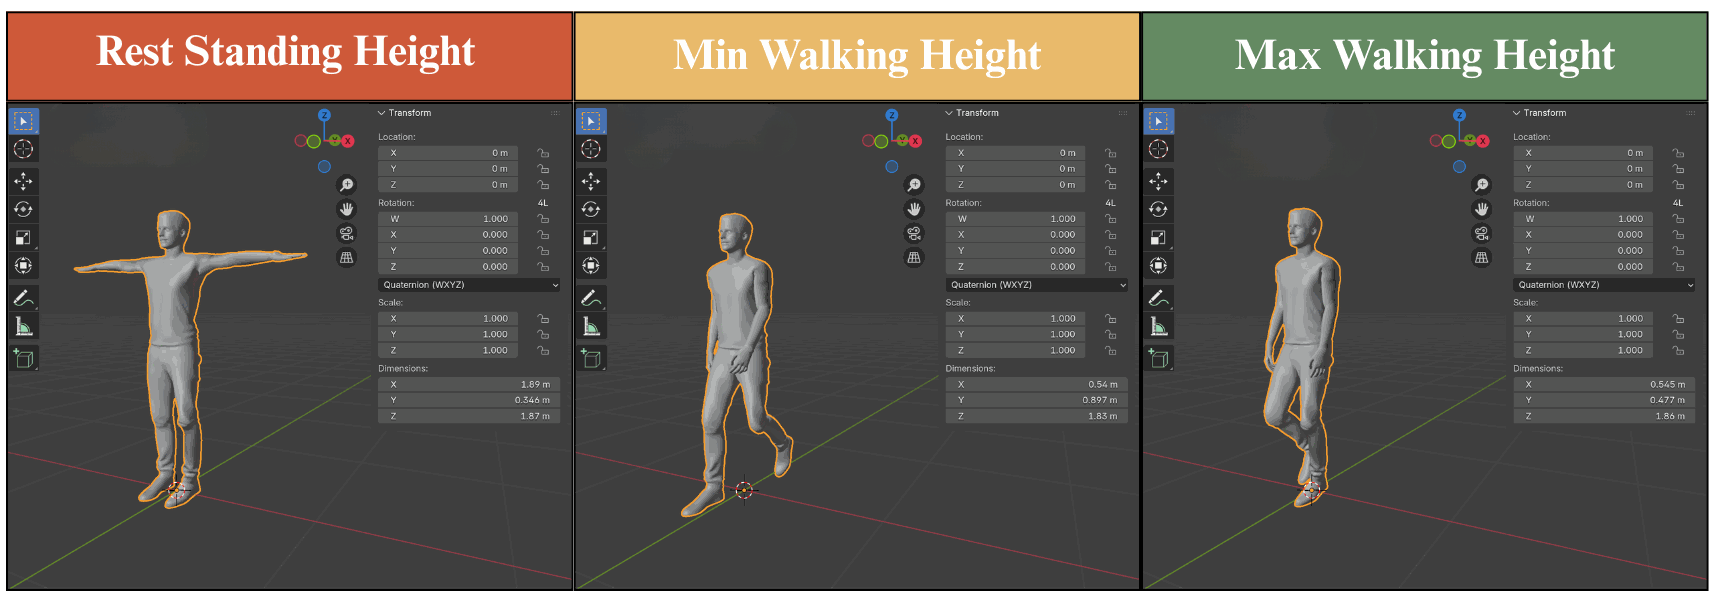
\includegraphics[width=0.99\linewidth]{sec/images/human_height_measure.png}
    \caption{\textbf{Examples of human height measuring.}}
    \label{fig:human_height_measure}
\end{figure*}

Similarly, for other rigged objects (such as birds and insects), we track their width frame by frame over the flight segment of the clip and only record the smallest and largest width observed. See details in \autoref{fig:bird_width_measure}. This is because, unlike the human case, these assets may not admit a clear, static “rest standing” pose in which the animal is fully extended. As a result, we do not define a separate rest measurement for flying objects.

\begin{figure*}[ht!]
    \centering
    \includegraphics[width=0.99\linewidth]{sec/images/bird_width.png}
    \caption{\textbf{Examples of flying animal measuring.}}
    \label{fig:bird_width_measure}
\end{figure*}

Correspondingly, the inference questions and prior ground truth are phrased with the same level of precision. For human figures, we explicitly distinguish between the standing height at rest and the minimum and maximum height observed while walking. For flying animals, we clearly refer to the minimum or maximum width attained during flight.

\subsubsection{Displacement or Path.} 

All displacement- or path-related labels are computed from object trajectories in Blender world space using internal custom Python scripts.

\noindent\textbf{Time--frame alignment across scenes.}
In Blender, each scene specifies a render range with \texttt{scene.frame\_start} and \texttt{scene.frame\_end}, and \texttt{scene.frame\_start} is not required to be 0. We define time \(t = 0\) to occur at the render start frame, regardless of its numeric index. More precisely, if a scene has frame rate \(f\) frames per second and render start frame \(f_{\text{start}}\), then the first frame of the exported video (timestamp \(t = 0\) s) is Blender frame \(f_{\text{start}}\), the frame at time \(t = 1/f\) s is frame \(f_{\text{start}} + 1\), and so on.

When a question specifies a time interval \([t_{\text{start}}, t_{\text{end}}]\) in seconds, we convert it to Blender frame indices by
\[
i_{\text{start}} = \mathrm{round}\bigl(f_{\text{start}} + f\, t_{\text{start}}\bigr),\quad
i_{\text{end}}   = \mathrm{round}\bigl(f_{\text{start}} + f\, t_{\text{end}}\bigr).
\]

This convention works uniformly for all scenes, including those whose render ranges begin at non-zero frame numbers (e.g., \texttt{frame\_start = 20, 40, 60, \dots}). In code, the conversion has the following form:

\begin{minted}[
fontsize=\footnotesize,
linenos,
frame=lines,
framesep=2mm,
baselinestretch=1.0,
breaklines,
bgcolor=black!2
]{python}
scene   = bpy.context.scene
fps     = scene.render.fps
f_start = scene.frame_start                      # may be 0, 20, 40, ...

def time_to_frame(t_sec: float) -> int:
    return round(f_start + t_sec * fps)
\end{minted}

When an interval is specified directly in frames, we simply take \((i_{\text{start}}, i_{\text{end}})\) as given and interpret the corresponding times as
\[
t_{\text{start}} = \frac{i_{\text{start}} - f_{\text{start}}}{f},\quad
t_{\text{end}}   = \frac{i_{\text{end}}   - f_{\text{start}}}{f},
\]
so that \(t = 0\) always aligns with the first frame of the rendered video, irrespective of the absolute Blender frame index.

At any frame \(i\), the scripts query the world-space position of the target object (e.g., the animated rigid body) via

\begin{minted}[
fontsize=\footnotesize,
linenos,
frame=lines,
framesep=2mm,
baselinestretch=1.0,
breaklines,
bgcolor=black!2
]{python}
scene.frame_set(i)
loc = obj.matrix_world.translation.copy()          # (x, y, z) in world space
\end{minted}

yielding a vector $p(i) = (x(i), y(i), z(i)) \in \mathbb{R}^3$.

\noindent\textbf{Displacement annotations.}
For displacement labels, we consider a time interval \([t_{\text{start}}, t_{\text{end}}]\)  or frame interval \([i_{\text{start}}, i_{\text{end}}]\). The scripts record the world-space locations
\[
p_{\text{start}} = p(t_{\text{start}}) = p(i_{\text{start}}),\quad
p_{\text{end}}   = p(t_{\text{end}})   = p(i_{\text{end}}),
\]
and form the displacement vector
\[
\Delta p = p_{\text{end}} - p_{\text{start}} = (\Delta x, \Delta y, \Delta z).
\]

From this vector we derive two scalar quantities.

\begin{enumerate}
    
\item The full 3D displacement
\[
D_{\text{3D}} = \lVert \Delta p \rVert_2 = \sqrt{\Delta x^2 + \Delta y^2 + \Delta z^2},
\]
\item The planar displacement in a 2D plane, obtained by projecting the motion onto that plane. 
For any chosen 2D coordinate plane with axes \((u, v)\), we define the planar displacement as
\[
D_{2\text{D}} = \sqrt{(\Delta u)^2 + (\Delta v)^2}.
\]
\end{enumerate}

In our benchmark we primarily use the three canonical planes:
the horizontal ground plane
\[
D_{\text{XY}} = \sqrt{(\Delta x)^2 + (\Delta y)^2},
\]
and the two vertical planes
\[
D_{\text{XZ}} = \sqrt{(\Delta x)^2 + (\Delta z)^2}, \qquad
D_{\text{YZ}} = \sqrt{(\Delta y)^2 + (\Delta z)^2}.
\]

A compact version of the core computation is:

\begin{minted}[
fontsize=\footnotesize,
linenos,
frame=lines,
framesep=2mm,
baselinestretch=1.0,
breaklines,
bgcolor=black!2
]{python}
def displacement_world(obj, frame_start, frame_end, scene):
    # sample world-space positions at start and end
    loc_start = get_world_location_at_frame(obj, frame_start, scene)
    loc_end   = get_world_location_at_frame(obj, frame_end, scene)

    # displacement vector
    disp_vec = loc_end - loc_start
    dx, dy, dz = disp_vec.x, disp_vec.y, disp_vec.z

    # 3D displacement and horizontal (XY) displacement
    D_3D = disp_vec.length                 # sqrt(dx*dx + dy*dy + dz*dz)
    D_XY = (dx**2 + dy**2) ** 0.5          # sqrt(dx*dx + dy*dy)

    return {
        "frame_start": frame_start,
        "frame_end": frame_end,
        "loc_start":  loc_start,
        "loc_end":    loc_end,
        "dx": dx, "dy": dy, "dz": dz,
        "D_3D": D_3D,
        "D_XY": D_XY,
    }
\end{minted}


For each annotated interval, we store:
\begin{itemize}
  \item the frame indices \((i_{\text{start}}, i_{\text{end}})\);
  \item the corresponding times \((t_{\text{start}}, t_{\text{end}})\), computed relative to the render start frame as above;
  \item the start and end world-space coordinates \(p_{\text{start}}, p_{\text{end}}\);
  \item the displacement components \((\Delta x, \Delta y, \Delta z)\);
  \item the two scalar values \(D_{\text{3D}}\) and \(D_{\text{XY}}\) in Blender units.
\end{itemize}

In the question text, we explicitly state whether “displacement” refers to the full 3D displacement \(D_{\text{3D}}\) or to a planar displacement \(D_{2\text{D}}\) in a specified plane (e.g., horizontal \(D_{\text{XY}}\) or vertical \(D_{\text{XZ}}\) / \(D_{\text{YZ}}\)). 
The posterior ground-truth answer for that question is taken from the corresponding stored value.


\subsubsection{Velocity and Acceleration.}

\noindent\textbf{Velocity measurement and uniform-speed diagnostics.}
Using the time--frame convention introduced above, let \(p_i \in \mathbb{R}^3\) denote the world-space origin of the target object at frame \(i\), obtained by querying \texttt{obj.matrix\_world.translation} after calling \texttt{scene.frame\_set(i)}. For two consecutive frames \(i-1\) and \(i\) with timestamps \(t_{i-1}\) and \(t_i\), we define the temporal spacing
\[
\Delta t_i = t_i - t_{i-1},
\]
and the instantaneous 3D velocity and scalar speed at frame \(i\) as
\[
\mathbf{v}_i = \frac{p_i - p_{i-1}}{\Delta t_i},
\qquad
s_i = \|\mathbf{v}_i\|_2,
\]
where \(\mathbf{v}_i = (v_{x,i}, v_{y,i}, v_{z,i})\) is the full 3D velocity vector in world coordinates and
\[
s_i = \lVert \mathbf{v}_i \rVert_2
= \sqrt{v_{x,i}^2 + v_{y,i}^2 + v_{z,i}^2}
\]
is its Euclidean norm. All operations are performed in Blender world space and use the true frame rate, so that positions \(p_i\), velocities \(\mathbf{v}_i\), and speeds \(s_i\) are expressed in a self-consistent system of physical units determined by the underlying scene scale.

The Blender analysis script computes these quantities frame by frame and writes them into a text block in Blender's Text Editor:
\begin{minted}[
fontsize=\footnotesize,
linenos,
frame=lines,
framesep=2mm,
baselinestretch=1.0,
breaklines,
bgcolor=black!2
]{python}
prev_loc   = None
prev_frame = None

for frame in range(frame_start, frame_end + 1):
    scene.frame_set(frame)
    loc = obj.matrix_world.translation.copy()   # p_i

    if prev_loc is None:
        vel_vec = Vector((0.0, 0.0, 0.0))
        speed   = 0.0
    else:
        dt      = (frame - prev_frame) / fps        # delta t_i
        disp    = loc - prev_loc                    # p_i - p_{i-1}
        vel_vec = disp / dt                         # v_i
        speed   = vel_vec.length                    # s_i

    write_per_frame_entry(frame, loc, vel_vec, speed)
    prev_loc   = loc
    prev_frame = frame
\end{minted}

For each frame \(i\) in the chosen range, this loop automatically prints one line of kinematic data into the text block, containing:
\begin{itemize}
  \item the frame index \(i\) and its timestamp \(t_i\) (relative to the render start frame);
  \item the world-space position \(p_i\);
  \item the full 3D velocity vector \(\mathbf{v}_i\);
  \item the scalar speed \(s_i\).
\end{itemize}
Any question that refers to “the speed at \(t\) seconds” or “the velocity at frame \(i\)” is answered by mapping the queried time to a frame index using the same time--frame conversion and then reading off the corresponding per-frame entry from this table, without any manual measurement or additional approximation.

In addition to per-frame velocities, we use the sequence of speeds \(\{s_i\}\) to characterize simple motion regimes at the clip level. Let \(I_v\) be the index set of frames for which a speed value is defined (all frames except the very first one), and let \(N_v = |I_v|\). We compute the mean speed
\[
\bar{s} = \frac{1}{N_v} \sum_{i \in I_v} s_i
\]
and the maximum relative deviation from this mean,
\[
\delta_{\text{speed}} =
\begin{cases}
0, & \text{if } \bar{s} = 0, \\[4pt]
\displaystyle \max_{i \in I_v} \frac{|s_i - \bar{s}|}{\bar{s}}, & \text{otherwise.}
\end{cases}
\]
Given a user-specified tolerance \(\tau_v\) (parameter \texttt{UNIFORM\_SPEED\_TOLERANCE}, e.g., \(\tau_v = 0.01\)), we classify the clip as:
\begin{itemize}
  \item \textbf{no effective motion} if \(\bar{s} \approx 0\) (numerically \(\bar{s} = 0\), indicating that the object is essentially stationary);
  \item \textbf{approximately uniform speed} if \(\bar{s} > 0\) and \(\delta_{\text{speed}} \le \tau_v\);
  \item \textbf{non-uniform speed} otherwise (speed fluctuations exceed the tolerance).
\end{itemize}
This logic matches the following code fragment:
\begin{minted}[
fontsize=\footnotesize,
linenos,
frame=lines,
framesep=2mm,
baselinestretch=1.0,
breaklines,
bgcolor=black!2
]{python}
avg_speed   = sum(speeds) / len(speeds)
max_dev     = max(abs(s - avg_speed) for s in speeds)
max_rel_dev = max_dev / avg_speed if avg_speed != 0 else 0.0

if avg_speed == 0:
    # almost no motion
    ...
else:
    if max_rel_dev <= UNIFORM_SPEED_TOLERANCE:
        # approximately uniform speed
        ...
    else:
        # not uniform-speed
        ...
\end{minted}

\noindent\textbf{Acceleration measurement and acceleration diagnostics.}
Starting from the third frame, we derive a scalar acceleration sequence that describes how quickly the object’s speed changes over time. Given the per-frame speeds \(\{s_i\}\) defined above, and the same temporal spacings \(\Delta t_i = t_i - t_{i-1}\), we define for all frames \(i \geq 2\)
\[
a_i = \frac{s_i - s_{i-1}}{\Delta t_i},
\]
so that \(a_i\) measures the finite-difference rate of change of speed between frames \(i-1\) and \(i\). The script computes these values alongside the speeds:
\begin{minted}[
fontsize=\footnotesize,
linenos,
frame=lines,
framesep=2mm,
baselinestretch=1.0,
breaklines,
bgcolor=black!2
]{python}
prev_speed = None
prev_frame = None

for frame in range(frame_start, frame_end + 1):
    scene.frame_set(frame)
    loc = obj.matrix_world.translation.copy()

    if prev_frame is None:
        dt    = 0.0
        speed = 0.0
        accel = None
    else:
        dt      = (frame - prev_frame) / fps
        disp    = loc - prev_loc
        vel_vec = disp / dt
        speed   = vel_vec.length

        if prev_speed is None:
            accel = None
        else:
            accel = (speed - prev_speed) / dt   # a_i

    write_per_frame_entry(frame, speed, accel)
    prev_loc   = loc
    prev_speed = speed
    prev_frame = frame
\end{minted}

For each frame \(i\) in the valid range, this produces a scalar acceleration value \(a_i\) (undefined at the first two frames), which we store in the same text table. Any question that refers to “the acceleration at frame \(i\)” or to “the acceleration over a given interval” is answered by mapping the queried time to a frame index and reading off the corresponding \(a_i\) entry.

To summarize acceleration behaviour over the entire clip, we perform an analogous diagnostic analysis on the set of defined accelerations. Let \(I_a\) be the index set of frames for which \(a_i\) is defined (starting from the third frame), and let \(N_a = |I_a|\). We compute the mean acceleration
\[
\bar{a} = \frac{1}{N_a} \sum_{i \in I_a} a_i
\]
and the maximum absolute deviation from this mean,
\[
\Delta_a^{\max} = \max_{i \in I_a} |a_i - \bar{a}|.
\]
If \(|\bar{a}|\) is larger than a small absolute threshold \(\varepsilon_{\min}\) (parameter \texttt{MIN\_ABS\_ACCEL}), we also measure the maximum relative deviation
\[
\delta_{\text{accel}} =
\begin{cases}
0, & \text{if } |\bar{a}| \le \varepsilon_{\min}, \\[4pt]
\displaystyle \frac{\Delta_a^{\max}}{|\bar{a}|}, & \text{otherwise.}
\end{cases}
\]
Given a user-specified tolerance \(\tau_a\) (parameter \texttt{UNIFORM\_ACCEL\_TOLERANCE}), the script then classifies the acceleration regime as:
\begin{itemize}
  \item \textbf{near-zero acceleration} if \(|\bar{a}| \le \varepsilon_{\min}\); in this case the overall acceleration is negligible and the clip is better interpreted as approximately constant-speed (or almost static);
  \item \textbf{approximately uniformly accelerated} if \(|\bar{a}| > \varepsilon_{\min}\) and \(\delta_{\text{accel}} \le \tau_a\); the sign of \(\bar{a}\) further distinguishes \emph{uniform acceleration} (\(\bar{a} > 0\)) from \emph{uniform deceleration} (\(\bar{a} < 0\));
  \item \textbf{irregular acceleration} otherwise, meaning that the accelerations fluctuate significantly around their mean.
\end{itemize}
This classification logic is implemented as:
\begin{minted}[
fontsize=\footnotesize,
linenos,
frame=lines,
framesep=2mm,
baselinestretch=1.0,
breaklines,
bgcolor=black!2
]{python}
avg_accel   = sum(accels) / len(accels)
max_dev_a   = max(abs(a - avg_accel) for a in accels)
if abs(avg_accel) > MIN_ABS_ACCEL:
    max_rel_dev_a = max_dev_a / abs(avg_accel)
else:
    max_rel_dev_a = 0.0

if abs(avg_accel) <= MIN_ABS_ACCEL:
    # acceleration is very small -> closer to uniform speed / almost static
    ...
else:
    if max_rel_dev_a <= UNIFORM_ACCEL_TOLERANCE:
        if avg_accel > 0:
            # approximately uniformly accelerating
            ...
        elif avg_accel < 0:
            # approximately uniformly decelerating
            ...
        else:
            # numerically close to zero
            ...
    else:
        # not uniformly accelerated
        ...
\end{minted}

These acceleration diagnostics never modify the underlying frame-level values \(\{a_i\}\), just as the velocity diagnostics never modify \(\{s_i\}\) or \(\{\mathbf{v}_i\}\). Instead, they provide a principled, threshold-based way to tag each clip as approximately constant-speed, uniformly accelerated, uniformly decelerated, or irregular, allowing us to phrase velocity- and acceleration-related questions at a level of precision that matches the actual motion regime present in each clip.


\subsubsection{Depth and Distance}

All geometric quantities used in our benchmark are computed directly inside Blender in world coordinates via a Python script that evaluates the scene frame by frame. The script reads the world-space transforms of selected entities, computes Euclidean distances, and logs a per-frame table into a Blender Text Editor text block. From this table, we derive two kinds of quantities: (i) depth metadata between objects and the camera, and (ii) inter-object distances in 3D and in projected 2D planes. 

\noindent\textbf{Depth metadata (object--camera).}
We extract depth values in Blender only as auxiliary geometric metadata,
not appearing in the inference question text or supervised targets. For any
object \(o\) with world-space position
\[
\mathbf{p}_t(o) = (x_t^o, y_t^o, z_t^o) \in \mathbb{R}^3
\]
and the active camera object with world-space origin
\[
\mathbf{p}_t^{\text{cam}} = (x_t^{\text{cam}}, y_t^{\text{cam}}, z_t^{\text{cam}}) \in \mathbb{R}^3,
\]
at time \(t\), we define the depth as the 3D Euclidean distance

\[
\begin{aligned}
d^{\text{depth}}_t(o)
&= \bigl\lVert \mathbf{p}_t(o) - \mathbf{p}_t^{\text{cam}} \bigr\rVert_2 \\
&= \sqrt{(x_t^o - x_t^{\text{cam}})^2 + (y_t^o - y_t^{\text{cam}})^2 + (z_t^o - z_t^{\text{cam}})^2}.
\end{aligned}
\]

During annotation, we treat \(d^{\text{depth}}_t(o)\) as a time series and often materialize it at a small set of shared reference time points (e.g., \(t_1 = 1\text{s}\), \(t_2 = 2\text{s}\)). Thus, for a moving object we record pairs such as
\[
\bigl(d^{\text{depth}}_{t_1}(o),\, d^{\text{depth}}_{t_2}(o)\bigr),
\]
and we use the same time points for other relevant entities in the scene (e.g., additional moving objects or candidate target objects). This temporal alignment ensures that when we expose depth values as priors, they are always comparable across objects at exactly the same timestamps. For static objects, the depth is constant over the clip, so the values at different time points are trivially identical.

Crucially, we never use these depth values as evaluation targets. We do not ask questions of the form “What is the distance between object \(o\) and the camera at time \(t\)?”, and we do not treat \(d^{\text{depth}}_t(o)\) as ground truth in any task. Instead, depth is used only as internal geometric metadata and, in some infer questions, as numeric priors that can help a VLM reason about the relative 3D configuration of the scene. Even in those infer questions, we do not necessarily expose the camera--target depth of the queried object itself; rather, we expose a subset of aligned depth values for selected objects. All exposed depth values are manually reviewed to ensure that, together with the visual information, they are logically sufficient to infer the correct answer.

\noindent\textbf{3D inter-object distances.}
We use the same Blender script to annotate 3D distances between pairs of entities. In our benchmark, these entities are either
(i) two moving objects, or
(ii) a moving object and a static reference object in the scene.
We do not treat object--camera distances as inter-object ground truth; camera-related distances only appear as depth metadata as described above.

Let $\mathbf{p}_t(a) = (x_t^a, y_t^a, z_t^a)
\quad\text{and}\quad
\mathbf{p}_t(b) = (x_t^b, y_t^b, z_t^b)$ denote the world-space positions of entities \(a\) and \(b\) at time \(t\). The 3D object--object distance is
\[
\begin{aligned}
d^{3\text{D}}_t(a,b)
&= \bigl\lVert \mathbf{p}_t(a) - \mathbf{p}_t(b) \bigr\rVert_2 \\
&= \sqrt{(x_t^a - x_t^b)^2 + (y_t^a - y_t^b)^2 + (z_t^a - z_t^b)^2}.
\end{aligned}
\]


For objects whose dimensions do not change over time, we take \(\mathbf{p}_t(o)\)to be the Blender object origin in world coordinates. For articulated skeletal models (e.g., humans), transformations are defined on a set of bones rather than a single rigid body. In these cases, we first enumerate all bones in the armature and select a semantically stable reference joint (for humans, typically the pelvis/hip bone) as the anchor. All distances involving that character are then defined using the world-space position of this reference bone, which provides a temporally stable and semantically meaningful notion of “where the character is”. For some non-humanoid articulated assets or composite rigs where no single point or bone has a clear semantic interpretation as the “character center” (e.g., certain vehicles or multi-part machines), we instead introduce an auxiliary helper object. Concretely, we create an Empty object \(h\) rigidly parented to the rig root, snap its origin to the root in world space, and log its world-space position \(\mathbf{p}_t(h)\) at each frame. In those scenes, all distances involving the articulated asset are computed with respect to \(\mathbf{p}_t(h)\) rather than a specific bone. This dual strategy (bone-based anchors for humanoid characters and helper-object anchors for other articulated assets) keeps the distance annotations consistent while accommodating the diversity of rig structures in our Blender scenes.

\noindent\textbf{Planar (2D) distances.}
Some tasks explicitly constrain distance reasoning to a 2D projection, for example ``horizontal distance in the ground plane'' or ``distance in the vertical cross-section''. To support such tasks, we also annotate \emph{planar distances} by projecting 3D positions onto a chosen coordinate plane \(\Pi \in \{\mathrm{XY}, \mathrm{XZ}, \mathrm{YZ}\}\). We define the projections
\[
\begin{aligned}
\Pi_{\mathrm{XY}}(x,y,z) &= (x,y),\\
\Pi_{\mathrm{XZ}}(x,y,z) &= (x,z),\\
\Pi_{\mathrm{YZ}}(x,y,z) &= (y,z).
\end{aligned}
\]
The planar distance between \(a\) and \(b\) at time \(t\) is then
\[
d^{\text{plane}}_t(a,b)
= \bigl\lVert \Pi\bigl(\mathbf{p}_t(a)\bigr) - \Pi\bigl(\mathbf{p}_t(b)\bigr) \bigr\rVert_2.
\]

Whether a distance question is treated as 2D or 3D in our benchmark is fully determined by (i) the infer question and (ii) the geometric category of the underlying video (2D vs.\ 3D sequence). Each video is assigned to a 2D or 3D split based on how it is generated and how its geometry is intended to be interpreted.

For videos in the 2D split, distances are interpreted in a single plane by construction. If a question in such a video simply asks for ``the distance between objects \(a\) and \(b\)'', the ground-truth target is the planar distance \(d^{\text{plane}}_t(a,b)\), and the task is labeled as 2D.

For videos in the 3D split, we have full world-space geometry. If the infer question explicitly restricts reasoning to a plane (e.g., ``horizontal distance'' or ``vertical distance''), we again use the planar distance \(d^{\text{plane}}_t(a,b)\) and label the task as 2D. Otherwise, distance questions on 3D videos default to the full 3D Euclidean distance \(d_t(a,b)\) defined above, and these tasks are labeled as 3D.

\noindent\textbf{Blender implementation and per-frame logging.}
All depth and distance quantities above are computed by a unified Blender Python script. For a specified frame range \([f_{\min}, f_{\max}]\), the script iterates over frames, queries world-space positions, computes distances, and writes a formatted table into a Blender Text Editor text block. The core of the script is:
\begin{minted}[
fontsize=\footnotesize,
linenos,
frame=lines,
framesep=2mm,
baselinestretch=1.0,
breaklines,
breakanywhere,
bgcolor=black!2
]{python}
import bpy
from mathutils import Vector

scene = bpy.context.scene
fps   = scene.render.fps

def world_pos(obj_or_bone):
    """Return world-space translation of an object or a specific bone."""
    # For regular objects:
    if hasattr(obj_or_bone, "matrix_world"):
        return obj_or_bone.matrix_world.to_translation()
    # For pose bones (e.g., armature.pose.bones["Hips"]):
    return obj_or_bone.matrix.to_translation()

for f in range(f_min, f_max + 1):
    scene.frame_set(f)

    # Example: distance between entities A and B
    p_a = world_pos(entity_a)
    p_b = world_pos(entity_b)

    # Full 3D distance in world coordinates
    dist_3d = (p_a - p_b).length

    # Example planar distance in the XY plane (horizontal separation):
    # other planes (XZ, YZ) are obtained analogously in the full script.
    p_a_xy = Vector((p_a.x, p_a.y, 0.0))
    p_b_xy = Vector((p_b.x, p_b.y, 0.0))
    dist_xy = (p_a_xy - p_b_xy).length

    # Timestamp (seconds), assuming t = 0 at f_min
    t = (f - f_min) / fps

    # Log one line (frame, time, 3D distance, XY-plane distance, ...)
    write_to_text_block(f, t, dist_3d, dist_xy)
\end{minted}

The same script is run with different choices of \texttt{entity\_a} and \texttt{entity\_b} to (i) record object--camera distances as depth metadata and (ii) generate object--object distance annotations. In the code listing above, we show the XY-plane case for concreteness. In practice, this block is used as a template: when planar distances in other coordinate planes (XZ or YZ) are
needed, we simply modify the projection lines accordingly (e.g.,\texttt{Vector((p\_a.x, p\_a.z, 0.0))} for XZ or
\texttt{Vector((0.0, p\_a.y, p\_a.z))} for YZ) and rerun the script for that scene.

All measurements are derived directly from Blender's world-space transforms, so the numeric values used in our questions and annotations match the underlying scene geometry exactly. Depth values are stored only as auxiliary geometric
metadata or optional numeric priors, whereas inter-object distances serve as the ground truth posterior.


\subsection{Lab Data Annotation}

Unlike Blender-based simulations, lab captures do not provide annotations that can be directly read out from software. Nevertheless, with our multi-stereo camera setup, we are able to reconstruct both the 3D scene and the 3D geometry of the target objects.

To obtain annotations for lab captures, we first attempted to use off-the-shelf 3D reconstruction models such as FoundationPose~\cite{wen2024foundationpose} to assist with annotation. However, in our experiments, we found that even state-of-the-art AI models struggled to localize objects stably in world coordinates and frequently failed under occlusions. 

Therefore, we instead rely on traditional geometry-based reconstruction with calibrated camera poses. We use the main camera together with manually selected metric depth values to recover the objects' world coordinates. Concretely, we use the UI-based annotation tool introduced earlier (see \autoref{fig:depth_annotator}) to manually click on the center of the target object across a sequence of frames in the video. The tool records the 2D coordinates of each click in image space together with the corresponding metric depth from the main camera. Using the calibrated camera intrinsics, we then back-project the annotated object centers into the world coordinate system.

To obtain static priors such as object size, we manually measure the shape and dimensions of each object to reduce measurement error. To obtain dynamic priors such as object velocities and accelerations, we annotate the object center across at least 5 adjacent frames (for smoothing purpose) and compute the instantaneous velocity and acceleration magnitudes from the resulting sequence of world coordinates, assuming a constant frame rate. Formally, the computation of dynamic priors in lab captured videos are:
\begin{align*}
v_k^{\mathrm{world}} 
  &\approx \frac{x_{k+1}^{\mathrm{world}} - x_{k}^{\mathrm{world}}}{\Delta t}, \\
a_k^{\mathrm{world}} 
  &\approx \frac{x_{k+1}^{\mathrm{world}} - 2 x_{k}^{\mathrm{world}} + x_{k-1}^{\mathrm{world}}}{\Delta t^2}, 
\end{align*}
where $\Delta t$ is determined from the frame rate of the captured videos.

Note that, based on our predefined questions and the priors required at specific time stamps, not all frames of the lab videos need to be annotated. This greatly reduces the annotation workload and helps prevent error accumulation over time.

When the object is occluded in the main camera view, we instead estimate its world coordinates by averaging the positions obtained by transforming its 2D annotations from the other three cameras into the world coordinate system.


\subsection{Internet Data Annotation}
\label{sec:internet_annotation}

For internet videos, we must derive kinematic ground truth from raw pixels rather than from simulator logs or calibrated sensors.
To keep the process systematic, we adopt a three-stage annotation workflow: (i) metadata and task specification, (ii) pixel-level measurement with a custom video tool, and (iii) conversion from pixel-space kinematics to real-world quantities.

\noindent\textbf{Metadata and task specification.}
Each collected internet clip is first assigned a unique identifier (e.g., \texttt{internet\_0001}).
Based on the scene content, annotators determine the physical prior available in the video (e.g., gravity $g=9.8\,\mathrm{m/s^2}$, the length of a credit card, lane width on a road, or conveyor-belt speed), and label the corresponding \textbf{\texttt{video\_type}} code (e.g., \texttt{S2MC}, \texttt{A2SS}) as described in \autoref{subsec:video_type}.
We then identify all feasible inference targets in the clip (e.g., vehicle speed, ball acceleration, object size) and enumerate kinematic inference questions that can be solved from the chosen prior.
For each question, we annotate the \textbf{\texttt{inference\_type}} (static vs.\ dynamic posterior) and write the final textual question so that the requested quantity, unit, and time reference (instantaneous vs.\ average) are explicit.

\begin{figure*}[ht!]
    \centering
    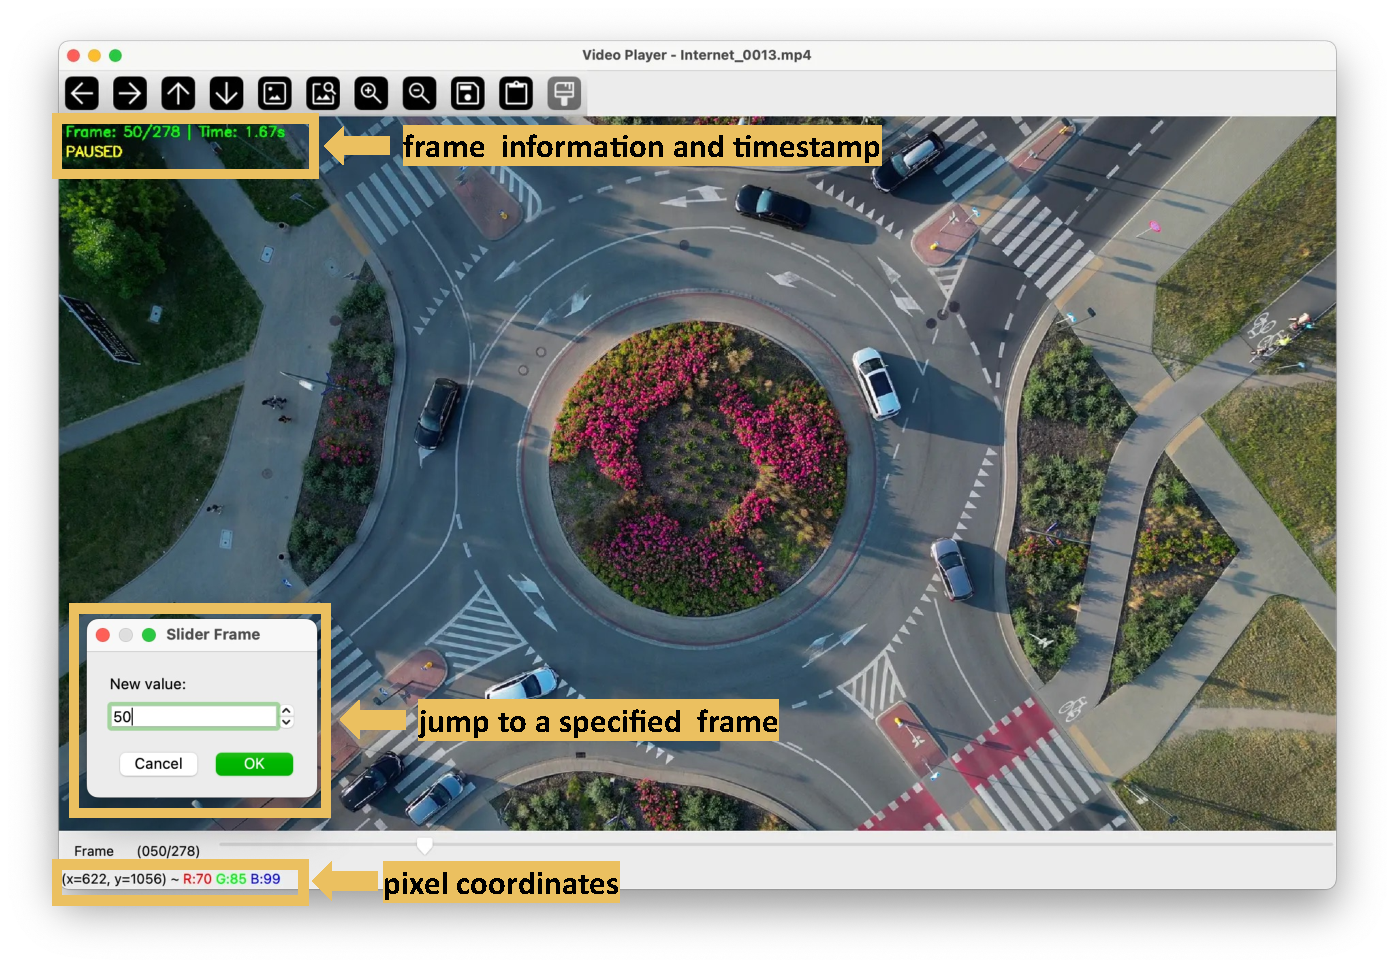
\includegraphics[width=0.99\linewidth]{sec/images/internet_parsing_ui.pdf}
    \caption{\textbf{Pixel-level measurement tool.}}
    \label{fig:internet_parsing}
\end{figure*}


\noindent\textbf{Pixel-level measurement tool.}
To read off pixel-space trajectories, we build a small annotation tool in Python using OpenCV.
The script takes as input the path to a video file and interactively queries the annotator for the correct frame rate.
It first shows the FPS detected by OpenCV, then allows the annotator to either accept it or manually enter a more reliable value (e.g., 24/25/30/60\,fps).
The tool verifies or manually counts the total frame number to avoid metadata errors, and reports basic properties such as resolution and duration.

After loading, the script launches an interactive player (\autoref{fig:internet_parsing}).
Each frame is overlaid with its index and timestamp, \texttt{ Frame: $k$/N | Time: $t_k$\,s}, and a play/pause status indicator.
A trackbar at the bottom allows direct jumping to any frame; dragging the slider or entering a frame index updates the display immediately.
Annotators can also step frame-by-frame with the left/right arrow keys or play the sequence in real time with the space bar.
In addition to these controls, we use a standard OpenCV mouse callback to display the current pixel coordinates $(x,y)$ of the cursor, which facilitates precise measurement of distances and object positions.


\noindent\textbf{(3) Measuring pixel-space kinematics.}
Given the verified frame rate $f$ (in fps), we set the time step as $\Delta t = 1/f$.
Annotators use the player to locate the relevant frames for each question:
for instantaneous quantities we jump to the frame closest to the target timestamp; for average quantities we select a sequence of frames spanning the interval of interest.
Along the main motion direction, we record
(i) the object’s pixel length $\mathbf S^{\mathrm{pixel}}$ (e.g., bumper-to-bumper for a car), and
(ii) the pixel coordinate $x_k^{\mathrm{pixel}}$ of the object’s reference point at discrete times
$t_k = k \Delta t$.

From these measurements we compute pixel-space kinematics using finite differences.
For a 1D trajectory $\{x_k^{\mathrm{pixel}}\}_{k=0}^{K}$, the (approximate) velocity and acceleration at time $t_k$ are
\begin{align*}
\mathbf V_k^{\mathrm{pixel}} 
  &\approx \frac{x_{k+1}^{\mathrm{pixel}} - x_{k}^{\mathrm{pixel}}}{\Delta t}, \\
\mathbf A_k^{\mathrm{pixel}} 
  &\approx \frac{x_{k+1}^{\mathrm{pixel}} - 2 x_{k}^{\mathrm{pixel}} + x_{k-1}^{\mathrm{pixel}}}{\Delta t^2}.
\end{align*}
When motion is measured in two image-plane directions, we apply the same formulas component-wise to $(x_k^{\mathrm{pixel}}, y_k^{\mathrm{pixel}})$.
In this way we obtain, for every prior object and inference target, the relevant pixel-space size $S^{\mathrm{pixel}}$, velocity $\mathbf V_k^{\mathrm{pixel}}$, and acceleration $\mathbf A_k^{\mathrm{pixel}}$.

\noindent\textbf{(4) Converting to real-world kinematics.}
Assuming planar motion (\autoref{sec:general_principles}), a single scalar scale factor $\gamma>0$ with units [world length / pixel] suffices along the motion direction.
Depending on which physical prior is available for a given clip, we estimate $\gamma$ via

\begin{equation*}
\gamma =
\begin{cases}
\dfrac{\mathbf S^{\mathrm{world}}}{\mathbf S^{\mathrm{pixel}}}, 
  & \text{if size prior is given} \\[0.6em]
\dfrac{\lvert \mathbf V^{\mathrm{world}}_{t_0} \rvert}{\lvert \mathbf V^{\mathrm{pixel}}_{t_0} \rvert},
  & \text{if velocity prior is given} \\[0.6em]
\dfrac{\lvert \mathbf A^{\mathrm{world}}_{t_0} \rvert}{\lvert \mathbf A^{\mathrm{pixel}}_{t_0} \rvert},
  & \text{if acceleration prior is given} \, .
\end{cases}
\label{eq:scale_factor}
\end{equation*}

where $t_0$ is the timestamp at which the prior is defined.

Once $s$ is determined, any kinematic quantity of the inference target can be expressed in world units by a simple rescaling:
\begin{align*}
(S_{\text{target}})^{\mathrm{world}} &= \gamma \, (S_{\text{target}})^{\mathrm{pixel}},\\
(\mathbf V_{\text{target}})^{\mathrm{world}}_{t_k} &= \gamma \, (\mathbf V_{\text{target}})^{\mathrm{pixel}}_{t_k},\\
(\mathbf A_{\text{target}})^{\mathrm{world}}_{t_k} &= \gamma \, (\mathbf A_{\text{target}})^{\mathrm{pixel}}_{t_k}.
\end{align*}
These world-space values are then used as the ground-truth priors and posteriors in \textsc{QuantiPhy}.




\subsection{Segmented Data}
Segmenting out target objects from the videos only changes the background and does not alter their original physical properties. Therefore, we reuse the original annotations of the videos for the segmented data without any modification.
